\documentclass[12pt,reqno,oneside]{amsart}
\usepackage{import}
%===============================%
%  Packages and basic settings  %
%===============================%
\usepackage[headheight=15pt,rmargin=0.5in,lmargin=0.5in,tmargin=0.75in,bmargin=0.75in]{geometry}
\usepackage{imakeidx}
\usepackage{framed}
\usepackage{amssymb}
\usepackage{amsmath}
\usepackage{mathrsfs}
\usepackage{enumitem}
\usepackage{hyperref}
\usepackage{appendix}
\usepackage[capitalise,noabbrev]{cleveref}
\usepackage{tikz}
\usepackage{tikz-cd}
\usepackage{nomencl}\makenomenclature
\usetikzlibrary{braids,arrows,decorations.markings,calc}

%====================================%
%  Theorems, environments & cleveref  %
%====================================%
\newtheorem{theorem}{Theorem}[section]
\newtheorem{proposition}{Proposition}[section]
\newtheorem{corollary}{Corollary}[section]
\newtheorem{lemma}{Lemma}[section]
\newtheorem{conjecture}{Conjecture}[section]
\newtheorem{remark}{Remark}[section]

\newenvironment{stabular}[2][1]
  {\def\arraystretch{#1}\tabular{#2}}
  {\endtabular}

%==================================%
%  Custom commands & environments  %
%==================================%
\newcommand{\legendre}[2]{\left(\frac{#1}{#2}\right)}
\newcommand{\dlegendre}[2]{\displaystyle{\left(\frac{#1}{#2}\right)}}
\newcommand{\tlegendre}[2]{\textstyle{\left(\frac{#1}{#2}\right)}}
\newcommand{\psum}{\sideset{}{'}\sum}
\newcommand{\asum}{\sideset{}{^{\ast}}\sum}
\newcommand{\tmod}[1]{\ \left(\text{mod }#1\right)}
\newcommand{\xto}[1]{\xrightarrow{#1}}
\newcommand{\xfrom}[1]{\xleftarrow{#1}}
\newcommand{\normal}{\mathrel{\unlhd}}
\newcommand{\mf}{\mathfrak}
\newcommand{\mc}{\mathcal}
\newcommand{\ms}{\mathscr}

\newcommand{\Mat}{\mathrm{Mat}}
\newcommand{\GL}{\mathrm{GL}}
\newcommand{\SL}{\mathrm{SL}}
\newcommand{\PSL}{\mathrm{PSL}}
\renewcommand{\O}{\mathrm{O}}
\newcommand{\SO}{\mathrm{SO}}
\newcommand{\U}{\mathrm{U}}
\newcommand{\Sp}{\mathrm{Sp}}

\newcommand{\N}{\mathbb{N}}
\newcommand{\Z}{\mathbb{Z}}
\newcommand{\Q}{\mathbb{Q}}
\newcommand{\R}{\mathbb{R}}
\newcommand{\C}{\mathbb{C}}
\newcommand{\F}{\mathbb{F}}
\renewcommand{\H}{\mathbb{H}}
\renewcommand{\P}{\mathbb{P}}

\renewcommand{\a}{\alpha}
\renewcommand{\b}{\beta}
\newcommand{\g}{\gamma}
\renewcommand{\d}{\delta}
\newcommand{\z}{\zeta}
\renewcommand{\t}{\theta}
\renewcommand{\i}{\iota}
\renewcommand{\k}{\kappa}
\renewcommand{\l}{\lambda}
\newcommand{\s}{\sigma}
\newcommand{\w}{\omega}

\newcommand{\G}{\Gamma}
\newcommand{\D}{\Delta}
\renewcommand{\L}{\Lambda}
\newcommand{\W}{\Omega}

\newcommand{\e}{\varepsilon}
\newcommand{\vt}{\vartheta}
\newcommand{\vphi}{\varphi}
\newcommand{\emt}{\varnothing}

\newcommand{\x}{\times}
\newcommand{\ox}{\otimes}
\newcommand{\op}{\oplus}
\newcommand{\bigox}{\bigotimes}
\newcommand{\bigop}{\bigoplus}
\newcommand{\del}{\partial}
\newcommand{\<}{\langle}
\renewcommand{\>}{\rangle}
\newcommand{\lf}{\lfloor}
\newcommand{\rf}{\rfloor}
\newcommand{\wtilde}{\widetilde}
\newcommand{\what}{\widehat}
\newcommand{\conj}{\overline}
\newcommand{\cchi}{\conj{\chi}}

\DeclareMathOperator{\id}{\textrm{id}}
\DeclareMathOperator{\sgn}{\mathrm{sgn}}
\DeclareMathOperator{\im}{\mathrm{im}}
\DeclareMathOperator{\rk}{\mathrm{rk}}
\DeclareMathOperator{\tr}{\mathrm{trace}}
\DeclareMathOperator{\nm}{\mathrm{norm}}
\DeclareMathOperator{\ord}{\mathrm{ord}}
\DeclareMathOperator{\Hom}{\mathrm{Hom}}
\DeclareMathOperator{\End}{\mathrm{End}}
\DeclareMathOperator{\Aut}{\mathrm{Aut}}
\DeclareMathOperator{\Tor}{\mathrm{Tor}}
\DeclareMathOperator{\Ann}{\mathrm{Ann}}
\DeclareMathOperator{\Gal}{\mathrm{Gal}}
\DeclareMathOperator{\Trace}{\mathrm{Trace}}
\DeclareMathOperator{\Norm}{\mathrm{Norm}}
\DeclareMathOperator{\Span}{\mathrm{Span}}
\DeclareMathOperator*{\Res}{\mathrm{Res}}
\DeclareMathOperator{\Vol}{\mathrm{Vol}}
\DeclareMathOperator{\Li}{\mathrm{Li}}
\renewcommand{\Re}{\mathrm{Re}}
\renewcommand{\Im}{\mathrm{Im}}

\newcommand{\GH}{\G\backslash\H}
\newcommand{\GG}{\G_{\infty}\backslash\G}

\newenvironment{psmallmatrix}
  {\left(\begin{smallmatrix}}
  {\end{smallmatrix}\right)}

%============%
%  Comments  %
%============%
\newcommand{\todo}[1]{\textcolor{red}{\sf Todo: [#1]}}

%===================%
%  Label reminders  %
%===================%
% [label=(\roman*)]
% [label=(\alph*)]
% [label=(\arabic{enumi})]

%==================%
%  Other settings  %
%==================%
\pgfdeclarelayer{background}
\pgfsetlayers{background,main}
\tikzset{->-/.style={decoration={
  markings,
  mark=at position .5 with {\arrow{>}}},postaction={decorate}}}

%=================%
%  Title & Index  %
%=================%
\title{A Multiple Dirichlet Series Approach to Shifted Convolution Sums}
\author{Henry Twiss}
\date{2024}
\makeindex

\begin{document}

\begin{abstract}
  A generalization of the classical additive divisor problem is that of shifted convolution sums for holomorphic cusp forms: find asymptotics for sums of the form
  \[
    S(X,h) = \sum_{1 < m \le X}A(m)\conj{B(m+h)},
  \]
  where $A(m)$ and $B(m)$ are the Hecke normalized Fourier coefficients of weight $k$ holomorphic cusp forms $f$ and $g$ on say $\PSL_{2}(\Z)\backslash\H$. One method of obtaining good estimates for $S(X,h)$ when $h \ge 1$ involves a detailed study of the spectral expansion of the shifted Dirichlet series
  \[
    D(s,h) = \sum_{m \ge 1}\frac{a(m)b(m+h)}{m^{s+k-1}},
  \]
  where $a(m)$ and $b(m)$ are the unnormalized Fourier coefficients. In the following, we discuss the analytic properties of the multiple Dirichlet series
  \[
    Z(s,w) = \sum_{m,h \ge 1}\frac{a(m)b(m+h)c(h)}{m^{s+k-1}h^{w+k-1}},
  \]
  where $c(h)$ are the Fourier coefficients of another weight $k$ holomorphic cusp form $l$. We exploit the analytic properties of this multiple Dirichlet series to sketch the proof of estimates for the following triple shifted convolution sums:
  \[
    T(X,Y) = \sum_{\substack{\frac{X}{2} < m \le X \\ \frac{Y}{2} < h \le Y}}A(m)B(m+h)C(h),
  \]
  where $C(h)$ are the Hecke normalized Fourier coefficients of $l$.
\end{abstract}

\maketitle

\section{Motivating Shifted Convolution Sums}
  The prototypical example of shifted convolution sums is when $a(m) = b(m) = \tau_{2}(n)$ is the usual divisor function. Obtaining estimates for the sum
  \[
    D_{2}(X,h) = \sum_{m \le X}\tau_{2}(m)\tau_{2}(m+h),
  \]
  is the well-known \textbf{binary additive divisor problem}. More generally, sums of the form
  \[
    D_{k,\ell}(X,h) = \sum_{m \le X}\tau_{k}(m)\tau_{\ell}(m+h),
  \]
  where $\tau_{k}$ is the $k$-th divisor function, are called \textbf{additive divisor sums}. These objects are of interest because $D_{k}(X,h) = D_{k,k}(X,h)$ is attached to the $2k$-th moment of the Riemann zeta function, defined by
  \[
    I_{k}(T) = \int_{0}^{T}\left|\z\left(\frac{1}{2}+it\right)\right|^{2k}\,dt.
  \]
  The first appearance of this phenomena occured in 1926 when Ingham (see \cite{I}) showed that $D_{2}(X,h)$ was related to the $4$-th moment by using estimate for $D_{2}(X,h)$ to establish the asymptotitc
  \[
    I_{2}(T) \sim \frac{T}{2\pi^{2}}(\log{T})^{4}. 
  \]
  The essential ingredient in Ingham's proof was an approximation function equation for $|\z\left(\frac{1}{2}+it\right)|^{4}$ involving the sums $D_{2}(X,h)$. Since Ingham's proof, many others have used results about additive divisor sums to establish asymptotics for moments (for example, see \cite{HB} and \cite{JM}). Unfortunately, not much is known about $D_{k}(X,h)$ when $k > 2$.
  
  On the other hand, when $k = 2$, additive divisor sums are also attached to the spectral theory of automorphic forms. This is because $\tau_{2}(m)$ appears as the $m$-th Fourier coefficeint of the Eisenstein series $E(z,s)$ on $\PSL_{2}(\Z)\backslash\H$ when $s = \frac{1}{2}$. When the $a(m)$ and $b(m)$ are Fourier coefficients of automorphic forms, the associated sum
  \[
    S(X,h) = \sum_{m \le X}A(m)B(m+h),
  \]
  with Hecke normalized Fourier coefficients, is called a \textbf{shifted convolution sum}. If the automorphic forms are non-cuspdial and the Fourier coefficients are Hecke normalized, we have
  \[
    S(X,h) = XP(\log(X))+O_{h,\e}(X^{\frac{2}{3}+\e}),
  \]
  where $P$ is some polynomial. Note that the error term here has cube root cancellation. Conjecturally, we should have square root cancellation in the error term (with an additional $h^{\e}$ factor). When the automorphic forms are cuspidal, there is no main term, but the error term is of the same size as in the non-cuspdial case. Again, the correct order of magnitude should have square root cancellation. The specific triple shifted convolution sums we will discuss below are when $a(m)$, $b(m)$, and $c(m)$, are Fourier coefficients of weight $k$ holomorphic cuspforms
  \[
    f(z) = \sum_{m \ge 1}a(m)e^{2\pi imz}, \quad g(z) = \sum_{m \ge 1}b(m)e^{2\pi imz}, \quad \text{and} \quad l(z) = \sum_{m \ge 1}c(m)e^{2\pi imz},
  \]
  on $\PSL_{2}(\Z)\backslash\H$. We will denote the Hecke normalized coefficients by $A(m)$, $B(m)$, and $C(m)$, respectively.
\section{Spectral Exapansions for Shifted Dirichlet Series}
  Let $h \ge 1$. We will estimate our shifted convolution sums using the shifted Dirichlet series
  \[
    D(s,h) = \sum_{m \ge 1}\frac{a(m)b(m+h)}{m^{s+k-1}}.
  \]
  The Ramanujan conjecture implies $a(m) \ll m^{\frac{k-1}{2}}$ and $b(m+h) \ll (m+h)^{\frac{k-1}{2}} \ll_{h} m^{\frac{k-1}{2}}$ and so $D(s,h)$ converges locally absolutely uniformly for $\Re(s) > 1$. It will be necessairy to analytically continue $D(s,h)$ to $\C$ and this is provided by its spectral exapansion. To obtain this spectral expansion, we consider a Poincar\'e series $P_{h,Y}(z,s;\d)$ which can be thought of as a $\d$-deformed version of the more classical  Poincar\'e $P_{h}(z,s)$ (studied by Selberg) and truncated outside of $Y^{-1} \le \Im(\g z) \le Y$. We compute $I_{Y,\d}(s,h)$ given by
  \[
    I_{Y,\d}(s,h) = \left\<P_{h,Y}(z,s;\d),f(z)\conj{g(z)}\Im(z)^{k}\right\>,
  \]
  in two ways. After unfolding and computing the spectral expansion, one analytically continutes $I_{Y,\d}(s,h)$. Upon taking the limit $Y \to \infty$, we arrive at
  \[
    I_{\d}(s,h) = \lim_{Y \to \infty}I_{Y,\d}(s,h) = \frac{\G(s+k-1)}{(4\pi)^{s+k-1}}D(s,h;\d),
  \]
  where $D(s,h;\d)$ is a $\d$-deformed version of $D(s,h)$ and $I_{\d}(s,h)$ admits a spectral exapansion. The analytic continuation of $I_{\d}(s,h)$ gives the analytic continuation of $D(s,h;\d)$ to all of $\C$. Taking the limit as $\d \to 0$ results in the analytic contunation of $D(s,h)$ to the region $\Re(s) < \frac{1-k}{2}$. A detailed derivation of the spectral expansion can be found in \cite{HH}. Explicitly, the spectral expansion modulo constants and the continuous spectrum is
  \begin{equation}\label{equ:spectral_exapansion_positive_case}
    D(s,h) = \sum_{t_{j}}h^{\frac{1}{2}-s}\conj{\rho_{j}(-h)}\frac{\G\left(1-s\right)\G\left(s-\frac{1}{2}+it_{j}\right)\G\left(s-\frac{1}{2}-it_{j}\right)}{\G\left(\frac{1}{2}+it_{j}\right)\G\left(\frac{1}{2}-it_{j}\right)\G(s+k-1)}\left\<u_{j}(z),f(z)\conj{g(z)}\Im(z)^{k}\right\>,
  \end{equation}
  which is valid when $\Re(s) < \frac{1-k}{2}$. Since $D(s,h) \ll 1$ for $\Re(s) > 1$, we see that $D(s,h)$ admits meromorphic continuation to $\C$ but we do not have an explicit expression for $D(s,h)$ in the strip $\frac{1-k}{2} \le \Re(s) \le 1$. As for residues, the residue of $D(s,h)$ at $s = \frac{1}{2}-\ell+it_{j}$ for $0 \le \ell \le \frac{k}{2}$ is
  \begin{equation}\label{equ:residue_of_shifted_Dirichlet}
    \Res_{s = \frac{1}{2}-\ell+it_{j}}D(s,h) = \frac{(-1)^{\ell}}{\ell!}\frac{\G(-\ell+2it_{j})\G\left(\frac{1}{2}+\ell-it_{j}\right)}{\G\left(\frac{1}{2}+it_{j}\right)\G\left(\frac{1}{2}-it_{j}\right)\G\left(k-\frac{1}{2}-\ell+it_{j}\right)}\frac{\conj{\rho_{j}(-h)}}{h^{it_{j}-\ell}} \cdot \left\<u_{j}(z),f(z)\conj{g(z)}\Im(z)^{k}\right\>.
  \end{equation}
  We also have an estimate in vertical strips. For $\frac{1-k}{2} \le \Re(s) \le 1$, there exists $N \ge 1$ such that
  \begin{equation}\label{equ:vertical_bound_shifted_Dirichlet_2}
    D(s,h) \ll_{\e} (1+|s|)^{N}h^{\frac{1}{2}+\t-\Re(s)+\e},
  \end{equation}
  where $\t$ is the best bound toward the Ramanujan-Petersson conjecture, provided $s$ is at least distance $\e$ away from the closest pole of $D(s,h)$.
\section{A Double Dirichlet Series for Shifted Convolution Sums}
  Let
  \[
    f(z) = \sum_{m \ge 1}a(m)e^{2\pi imz} \quad \text{and} \quad g(z) = \sum_{m \ge 1}b(m)e^{2\pi imz} \quad \text{and} \quad l(z) = \sum_{m \ge 1}c(m)e^{2\pi imz},
  \]
  be weight $k$ holomorphic cusp forms on $\G = \PSL_{2}(\Z)\backslash\H$. Define the double Dirichlet series
  \[
    Z(s,w) = \sum_{m,h \ge 1}\frac{a(m)b(m+h)c(h)}{m^{s+k-1}h^{w+k-1}} = \sum_{h \ge 1}\frac{D(s,h)c(h)}{h^{w+k-1}} = \sum_{m \ge 1}\frac{a(m)D(w,m)}{m^{s+k-1}}.
  \]
  As either of the latter two expressions converge absolutely uniformly on compacta provided $\Re(s) > 1$ and $\Re(w) > 1$, we see that $Z(s,w)$ is converges locally absolutely uniformly convergence in the region $\L_{0} = \{(s,w) \in \C^{2}:\Re(s) > 1, \Re(w) > 1\}$ and all of the equalities are justified. The last equality deserves as special name and is known as \textbf{the interchange} for $Z(s,w)$:
  \[
    \sum_{h \ge 1}\frac{D(s,h)c(h)}{h^{w+k-1}} = \sum_{m \ge 1}\frac{a(m)D(w,m)}{m^{s+k-1}}.
  \]
  Representing the point $(s,w)$ by $(\Re(s),\Re(w))$, graphically we have continuation to the region

  \begin{center}
    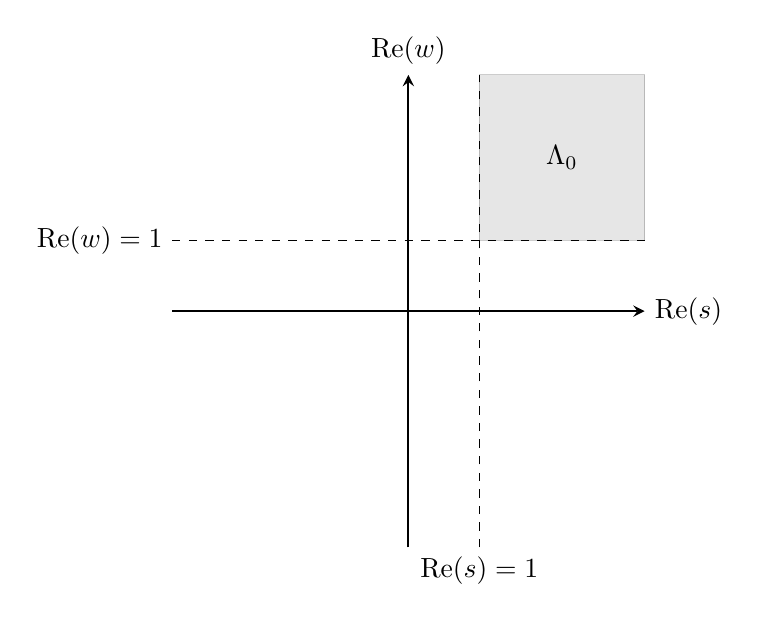
\begin{tikzpicture}[scale=3]
      \draw[thick,-stealth] (-1,0) -- (1,0) node [right] {$\Re(s)$};
      \draw[thick,-stealth] (0,-1) -- (0,1) node [above] {$\Re(w)$};

      \draw[fill=gray,opacity=0.2] (0.3,0.3) -- (1,0.3) -- (1,1) -- (0.3,1) -- cycle;

      \draw[dashed] (0.3,-1) -- (0.3,1);
      \draw[dashed] (-1,0.3) -- (1,0.3);

      \node at (0.65,0.65) {$\L_{0}$};
      \node at (0.3,-1) [below] {$\Re(s) = 1$};
      \node at (-1,0.3) [left] {$\Re(w) = 1$};
    \end{tikzpicture}
  \end{center}

  To obtain meromorphic continuation to a larger region in $s$, suppose $\Re(s) < \frac{1-k}{2}$ and replace $D(s,h)$ with its spectral expansion (modulo constants and the continuous spectrum) given in \cref{equ:spectral_exapansion_positive_case} to obtain
  \[
    Z(s,w) = \sum_{h \ge 1}\sum_{t_{j}}h^{\frac{1}{2}-s}\conj{\rho_{j}(-h)}\frac{\G\left(1-s\right)\G\left(s-\frac{1}{2}+it_{j}\right)\G\left(s-\frac{1}{2}-it_{j}\right)}{\G\left(\frac{1}{2}+it_{j}\right)\G\left(\frac{1}{2}-it_{j}\right)\G(s+k-1)}\left\<u_{j}(z),f(z)\conj{g(z)}\Im(z)^{k}\right\>\frac{c(h)}{h^{w+k-1}},
  \]
  Interchanging sums and collecting terms yields
  \[
    Z(s,w) = \sum_{t_{j}}\frac{\G\left(1-s\right)\G\left(s-\frac{1}{2}+it_{j}\right)\G\left(s-\frac{1}{2}-it_{j}\right)}{\G\left(\frac{1}{2}+it_{j}\right)\G\left(\frac{1}{2}-it_{j}\right)\G(s+k-1)}\left\<u_{j}(z),f(z)\conj{g(z)}\Im(z)^{k}\right\>\sum_{h \ge 1}\frac{\conj{\rho_{j}(-h)}c(h)}{h^{s+w+k-\frac{3}{2}}}.
  \]
  Now the sum over $h$ is the Rankin-Selberg convolution of $l$ and $u_{j}$ up to a zeta factor. Indeed,
  \[
    L(s,u_{j} \ox l) = \z(2s)\sum_{h \ge 1}\frac{\conj{\rho_{j}(-h)}C(h)}{h^{s}} = \z(2s)\sum_{h \ge 1}\frac{\conj{\rho_{j}(-h)}c(h)}{h^{s+\frac{k-1}{2}}},
  \]
  so that
  \[
    L\left(s+w+\frac{k}{2}-1,u_{j} \ox l\right) = \z(2s+2w+k-2)\sum_{h \ge 1}\frac{\conj{\rho_{j}(-h)}c(h)}{h^{s+w+k-\frac{3}{2}}}.
  \]
  This $L$-function admits analytic continuation to $\C$. Moreover, as the zeta factor has no zeros provided $\Re(2s+2w+k-2) > 1$, it follows that the sum over $h$ is holomorphic for $\Re\left(s+w+\frac{k}{2}-1\right) > \frac{1}{2}$ or equivalently $\Re(s+w) > \frac{3-k}{2}$. Therefore $Z(s,w)$ admits meromorphic continuation to the region
  \[
    \L_{s}' = \L_{0} \cup \left\{(s,w) \in \C^{2}:\Re\left(s+w\right) > \frac{3-k}{2}, \Re(s) < \frac{1-k}{2}\right\},
  \]
  where in the region $\L_{s}'-\L_{0}$, $Z(s,w)$ can be expressed as
  \[
    Z(s,w) = \sum_{t_{j}}\frac{\G\left(1-s\right)\G\left(s-\frac{1}{2}+it_{j}\right)\G\left(s-\frac{1}{2}-it_{j}\right)}{\G\left(\frac{1}{2}+it_{j}\right)\G\left(\frac{1}{2}-it_{j}\right)\G(s+k-1)}\left\<u_{j}(z),f(z)\conj{g(z)}\Im(z)^{k}\right\>\frac{L\left(s+w+\frac{k}{2}-1,u_{j} \ox l\right)}{\z(2s+2w+k-2)}.
  \]

  \begin{center}
    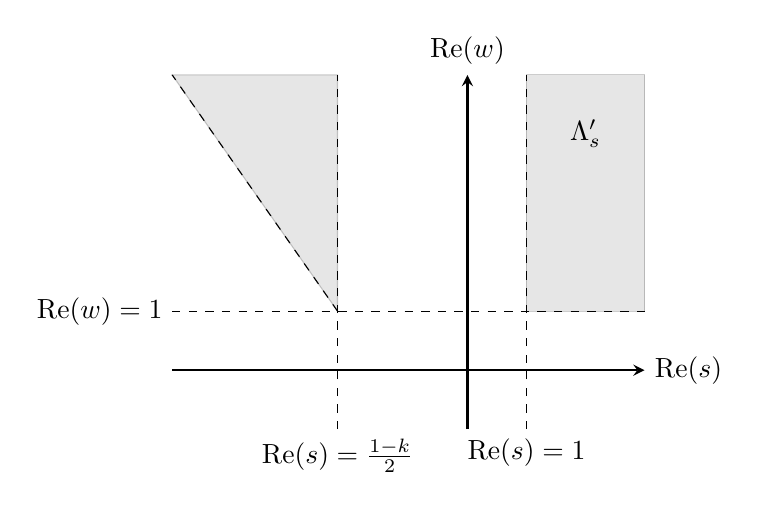
\begin{tikzpicture}[scale=3]
      \draw[thick,-stealth] (-1,-0.75) -- (1,-0.75) node [right] {$\Re(s)$};
      \draw[thick,-stealth] (0.25,-1) -- (0.25,0.5) node [above] {$\Re(w)$};

      \draw[fill=gray,opacity=0.2] (0.5,-0.5) -- (1,-0.5) -- (1,0.5) -- (0.5,0.5) -- cycle;

      \draw[fill=gray,opacity=0.2] (-0.3,-0.5) -- (-1,0.5) -- (-0.3,0.5) -- cycle;

      \draw[dashed] (0.5,-1) -- (0.5,0.5);
      \draw[dashed] (-1,-0.5) -- (1,-0.5);
      \draw[dashed] (-0.3,-1) -- (-0.3,0.5);
      \draw[dashed] (-0.3,-0.5) -- (-1,0.5);

      \node at (0.75,0.25) {$\L_{s}'$};
      \node at (0.5,-1) [below] {$\Re(s) = 1$};
      \node at (-1,-0.5) [left] {$\Re(w) = 1$};
      \node at (-0.3,-1) [below] {$\Re(s) = \frac{1-k}{2}$};
    \end{tikzpicture}
  \end{center}
  We can actually obtain continuation to a slightly large region at the expense of an explicit formula. To see this, using \cref{equ:vertical_bound_shifted_Dirichlet_2} we have
  \[
    Z(s,w) \ll_{\e} \sum_{h \ge 1}\frac{(1+|s|)^{N}c(h)}{h^{\Re(s+w)+k-\t-\e-\frac{3}{2}}},
  \]
  for $\frac{1-k}{2} < \Re(s) < 1$ and $\Re(w) > 1$ provided $s$ is at least distance $\e$ away from the closest pole. The latter expression converges in this region if $\Re(s+w) > \frac{5}{2}-k+\t+\e$, or equivalently, $k > 2+\t+\e$ wich holds because $k \ge 4$ and $\t < 1$. Since $D(s,h)$ admits meromorphic continuation to $\C$, the above bound implies that we obtain continuation to the region
  \[
    \L_{s} = \L_{0} \cup \left\{(s,w) \in \C^{2}:\Re\left(s+w\right) > \frac{3}{2}, \Re(w) > 1\right\}.
  \]

  \begin{center}
    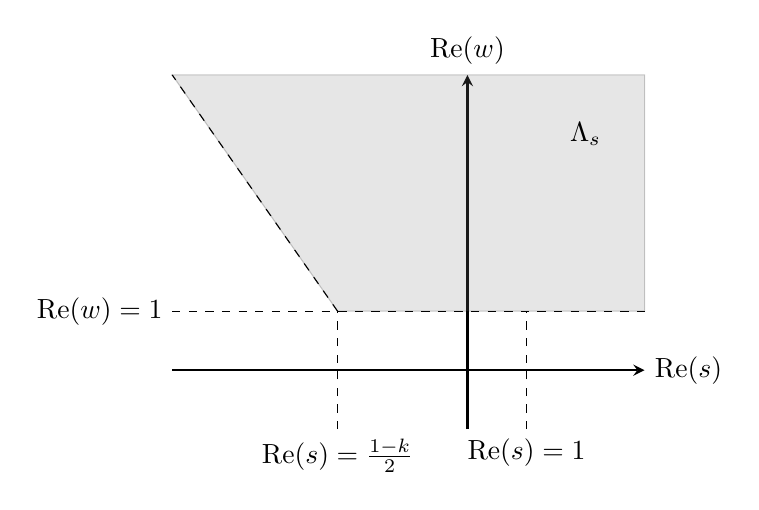
\begin{tikzpicture}[scale=3]
      \draw[thick,-stealth] (-1,-0.75) -- (1,-0.75) node [right] {$\Re(s)$};
      \draw[thick,-stealth] (0.25,-1) -- (0.25,0.5) node [above] {$\Re(w)$};

      \draw[fill=gray,opacity=0.2] (-0.3,-0.5) -- (-1,0.5) -- (1,0.5) -- (1,-0.5) -- (0.5,-0.5) -- (0.5,-0.5) -- cycle;

      \draw[dashed] (0.5,-1) -- (0.5,-0.5);
      \draw[dashed] (-1,-0.5) -- (1,-0.5);
      \draw[dashed] (-0.3,-1) -- (-0.3,-0.5);
      \draw[dashed] (-0.3,-0.5) -- (-1,0.5);

      \node at (0.75,0.25) {$\L_{s}$};
      \node at (0.5,-1) [below] {$\Re(s) = 1$};
      \node at (-1,-0.5) [left] {$\Re(w) = 1$};
      \node at (-0.3,-1) [below] {$\Re(s) = \frac{1-k}{2}$};
    \end{tikzpicture}
  \end{center}

  Using the interchange, we can perform the same procedure with the roles of $s$ and $w$ flipped to obtain meromorphic continuation to the region
  \[
    \L_{w}' = \L_{0} \cup \left\{(s,w) \in \C^{2}:\Re\left(s+w\right) > \frac{3-k}{2}, \Re(w) < \frac{1-k}{2}\right\},
  \]
  and hence to the larger region
  \[
    \L_{w} = \L_{0} \cup \left\{(s,w) \in \C^{2}:\Re\left(s+w\right) > \frac{3-k}{2}, \Re(s) > 1\right\}.
  \]
  Since the region $\L = \L_{s} \cup \L_{w}$ is a connected tube domain, we can appeal to Bochner's continuation theorem to at last obtain meromorphic continuation to the convex hull $\what{\L}$.

  \begin{center}
    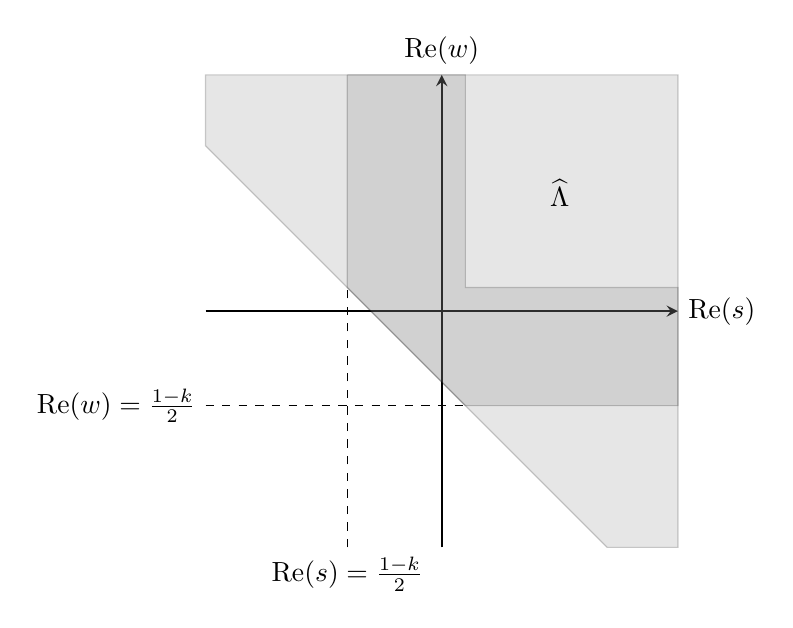
\begin{tikzpicture}[scale=3]
      \draw[thick,-stealth] (-1,0) -- (1,0) node [right] {$\Re(s)$};
      \draw[thick,-stealth] (0,-1) -- (0,1) node [above] {$\Re(w)$};

      \draw[fill=gray,opacity=0.2] (1,1) -- (-1,1) -- (-1,0.7) -- (0.7,-1) -- (1,-1) -- cycle;

      \draw[dashed] (-0.4,-1) -- (-0.4,0.1);
      \draw[dashed] (-1,-0.4) -- (0.1,-0.4);

      \draw[fill=gray,opacity=0.2] (-0.4,1) -- (-0.4,0.1) -- (0.1,-0.4) -- (1,-0.4) -- (1,0.1) -- (0.1,0.1) -- (0.1,1) -- (-0.4,1);

      \node at (0.5,0.5) {$\what{\L}$};
      \node at (-0.4,-1) [below] {$\Re(s) = \frac{1-k}{2}$};
      \node at (-1,-0.4) [left] {$\Re(w) = \frac{1-k}{2}$};
    \end{tikzpicture}
  \end{center}

  The primary benifit of meromorphic continuation to $\what{\L}$ is that we obtain continuation in a region containing the poles at $s = \frac{1}{2}+it_{j}$ (or $w = \frac{1}{2}+it_{j}$) provided $w$ (or $s$) has large enough real part. In particular, the representations
  \begin{align*}
    Z(s,w) &= \sum_{m,h \ge 1}\frac{a(m)b(m+h)c(h)}{m^{s+k-1}h^{s+k-1}}, \\
    Z(s,w) &= \sum_{t_{j}}\frac{\G\left(1-s\right)\G\left(s-\frac{1}{2}+it_{j}\right)\G\left(s-\frac{1}{2}-it_{j}\right)}{\G\left(\frac{1}{2}+it_{j}\right)\G\left(\frac{1}{2}-it_{j}\right)\G(s+k-1)}\left\<u_{j}(z),f(z)\conj{g(z)}\Im(z)^{k}\right\>\frac{L\left(s+w+\frac{k}{2}-1,u_{j} \ox l\right)}{\z(2s+2w+k-2)}, \\
    Z(s,w) &= \sum_{t_{j}}\frac{\G\left(1-w\right)\G\left(w-\frac{1}{2}+it_{j}\right)\G\left(w-\frac{1}{2}-it_{j}\right)}{\G\left(\frac{1}{2}+it_{j}\right)\G\left(\frac{1}{2}-it_{j}\right)\G(w+k-1)}\left\<u_{j}(z),f(z)\conj{g(z)}\Im(z)^{k}\right\>\frac{L\left(s+w+\frac{k}{2}-1,u_{j} \ox l\right)}{\z(2s+2w+k-2)},
  \end{align*}
  are valid on the corresponding regions
  \begin{align*}
      \L_{0} &= \{(s,w) \in \C^{2}:\Re(s) > 1, \Re(w) > 1\}, \\
      \L_{s}'-\L_{0} &= \cup \left\{(s,w) \in \C^{2}:\Re\left(s+w\right) > \frac{3-k}{2}, \Re(s) < \frac{1-k}{2}\right\}, \\
      \L_{w}'-\L_{0} &= \cup \left\{(s,w) \in \C^{2}:\Re\left(s+w\right) > \frac{3-k}{2}, \Re(s) < \frac{1-k}{2}\right\},
  \end{align*}
  and in general, $Z(s,w)$ admits meromorphic continuation to the region
  \[
    \what{\L} = \left\{(s,w) \in \C^{2}:\Re(s+w) > \frac{3-k}{2}\right\}.
  \]
  Accordingly, the darker shaded region in the figure above is exactly where we have meromorphic continuation of $Z(s,w)$ but do not have an expression for $Z(s,w)$. This region is
  \[
    \what{\L}-\L_{s}'-\L_{w}',
  \]
  and it includes some of the poles of $Z(s,w)$. In general, the poles of the shifted Dirichlet series $D(s,h)$ and $D(w,m)$ induce poles of $Z(s,w)$. No additional poles arise from the Rankin-Selberg convolutions appearing in the meromorphic continuation. Indeed, these convolutions are of a Maass cusp form and a modular form which are orthogonal with respect to the Petersson inner product. Let us compute the residue of $Z(s,w)$ at $s = \frac{1}{2}-\ell+it_{j}$ where $0 \le \ell \le \frac{k}{2}$ provided $\Re(w) > 1$. We use the representation
  \[
    Z(s,w) = \sum_{h \ge 1}\frac{D(s,h)c(h)}{h^{w+k-1}}.
  \]
  As each term in the numerator has a pole at $s = \frac{1}{2}-\ell+it_{j}$ via the spectral expansion, using \cref{equ:residue_of_shifted_Dirichlet} we obtain
  \begin{equation}\label{equ:residue_of_double_Dirichlet_series_1}
    \begin{aligned}
      \Res_{s = \frac{1}{2}-\ell+it_{j}}Z(s,w) &= \sum_{h \ge 1}\frac{(-1)^{\ell}}{\ell!}\frac{\G(-\ell+2it_{j})\G\left(\frac{1}{2}+\ell-it_{j}\right)}{\G\left(\frac{1}{2}+it_{j}\right)\G\left(\frac{1}{2}-it_{j}\right)\G\left(k-\frac{1}{2}-\ell+it_{j}\right)}\frac{\conj{\rho_{j}(-h)}c(h)}{h^{w+k-1-\ell+it_{j}}} \\
    &\cdot \left\<u_{j}(z),f(z)\conj{g(z)}\Im(z)^{k}\right\>,
    \end{aligned}
  \end{equation}
  Collecting the sum over $h$ gives the simplified expression
  \begin{equation}\label{equ:residue_of_double_Dirichlet_series_2}
    \begin{aligned}
      \Res_{s = \frac{1}{2}-\ell+it_{j}}Z(s,w) &= \frac{(-1)^{\ell}}{\ell!}\frac{\G(-\ell+2it_{j})\G\left(\frac{1}{2}+\ell-it_{j}\right)}{\G\left(\frac{1}{2}+it_{j}\right)\G\left(\frac{1}{2}-it_{j}\right)\G\left(k-\frac{1}{2}-\ell+it_{j}\right)}\frac{L\left(\frac{1}{2}-\ell+it_{j}+w+\frac{k}{2}-1,u_{j} \ox l\right)}{\z(1-2\ell+2it_{j}+2w+k-2)} \\
      &\cdot \left\<u_{j}(z),f(z)\conj{g(z)}\Im(z)^{k}\right\>,
      \end{aligned}
  \end{equation}
  The poles at $w = \frac{1}{2}+it_{j}$ are computed in the exact same was since $Z(s,w)$ is completely symmetric in $s$ and $w$.
\section{An Estimate for Short Sums}
  We will estimate sums of the form
  \[
    T(X,Y) = \sum_{\substack{\frac{X}{2} < m \le X \\ \frac{Y}{2} < h \le Y}}A(m)B(m+h)C(h),
  \]
  and show that they exhibit square root cancellation. First, we require an analytic expression for sums of the form
  \[
    T(X,h) = \sum_{\frac{X}{2} < m \le X}A(m)B(m+h),
  \]
  for fixed $h \ge 1$. We will assume we are working in the region of absolute uniform convergence on compacta of $Z(s,w)$. Let $\psi(t):[0,\infty) \to [0,\infty)$ be a bump function that is identically $1$ for $\frac{1}{2} < t \le 1$ and exhibits smooth exponential decay to zero in a unit interval outside of $\big(\frac{1}{2},1\big]$. Denote its Mellin transform by $\Psi(s)$. Then
  \[
    T(X,h) = \sum_{m \ge 1}A(m)B(m+h)\psi\left(\frac{m}{X}\right),
  \]
  and the smoothed version of Perron's formula give
  \begin{equation}\label{equ:Perron_for_double_sum_1}
    T(X,h) = \frac{1}{2\pi i}\int_{(2)}\sum_{m \ge 1}\frac{a(m)b(m+h)}{m^{s+\frac{k-1}{2}}(m+h)^{\frac{k-1}{2}}}\Psi(s)X^{s}\,ds.
  \end{equation}
  Recall the identity,
  \begin{equation}\label{equ:Mellin_inverse_gamma_ratio_identity}
    \frac{1}{(1+t)^{\b}} = \frac{1}{2\pi i}\int_{(c)}\frac{\G(\b-u)\G(u)}{\G(\b)}t^{-u}\,du,
  \end{equation}
  for any $0 < c < \b$. Pulling out a factor of $m^{\frac{k-1}{2}}$ in the denominator of \cref{equ:Perron_for_double_sum_1} and using \cref{equ:Mellin_inverse_gamma_ratio_identity} with $t = \frac{h}{m}$, $\b = \frac{k-1}{2}$, and $c = \e$ gives
  \begin{equation}\label{equ:Perron_for_double_sum_2}
    T(X,h) = \frac{1}{(2\pi i)^{2}}\int_{(\e)}\int_{(2)}\sum_{m \ge 1}\frac{a(m)b(m+h)}{m^{s-u+k-1}h^{u}}\frac{\G\left(\frac{k-1}{2}-u\right)\G(u)}{\G\left(\frac{k-1}{2}\right)}\Psi(s)X^{s}\,ds\,du.
  \end{equation}
  We can use this analytic expression for $T(X,h)$ to obtain one for $T(X,Y)$. First observe that
  \[
    T(X,Y) = \sum_{\frac{Y}{2} < h \le Y}T(X,h)C(h) = \sum_{h \ge 1}T(X,h)C(h)\psi\left(\frac{h}{Y}\right).
  \]
  Applying the smoothed version of Perron's formula again, and using \cref{equ:Perron_for_double_sum_2}, yields
  \begin{equation}\label{equ:Perron_for_triple_sum_1}
    T(X,Y) = \frac{1}{(2\pi i)^{3}}\int_{(\e)}\int_{(2)}\int_{(2)}\sum_{m \ge 1}\frac{a(m)b(m+h)c(h)}{m^{s-u+k-1}h^{w+u+\frac{k-1}{2}}}\frac{\G\left(\frac{k-1}{2}-u\right)\G(u)}{\G\left(\frac{k-1}{2}\right)}\Psi(s)\Psi(w)X^{s}Y^{w}\,ds\,dw\,du.
  \end{equation}
  In terms of $Z(s,w)$, \cref{equ:Perron_for_triple_sum_1} is expressed as
  \begin{equation}\label{equ:Perron_for_triple_sum_2}
    T(X,Y) = \frac{1}{(2\pi i)^{3}}\int_{(\e)}\int_{(2)}\int_{(2)}Z\left(s-u,w+u-\frac{k-1}{2}\right)\frac{\G\left(\frac{k-1}{2}-u\right)\G(u)}{\G\left(\frac{k-1}{2}\right)}\Psi(s)\Psi(w)X^{s}Y^{w}\,ds\,dw\,du.
  \end{equation}
  We will estimate this triple integral by shifting lines of integration. First, shift the line $(2)$ at $s$ to $\left(\frac{1}{2}\right)$. We pass poles coming from the multiple Dirichlet series when $s = \frac{1}{2}+u+it_{j}$ so that
  \begin{align*}
    T(X,Y) &= \frac{1}{(2\pi i)^{3}}\int_{(\e)}\int_{(2)}\int_{\left(\frac{1}{2}\right)}Z\left(s-u,w+u-\frac{k-1}{2}\right)\Psi(s)\Psi(w)X^{s}Y^{w}\,ds\,dw\,du \\
    &+ \frac{1}{(2\pi i)^{2}}\int_{(\e)}\int_{(2)}\sum_{t_{j}}R_{s}\left(w+u-\frac{k-1}{2},u;0,t_{j}\right)\Psi\left(\frac{1}{2}+it_{j}+u\right)\Psi(w)X^{\frac{1}{2}+u+it_{j}}Y^{w}\,dw\,du,
  \end{align*}
  where, using \cref{equ:residue_of_double_Dirichlet_series_2}, we have
  \begin{align*}
    R_{s}(w,u;\ell,t_{j}) &= \left[\Res_{s = \frac{1}{2}-\ell+it_{j}}Z(s,w)\right]\frac{\G\left(\frac{k-1}{2}-u\right)\G(u)}{\G\left(\frac{k-1}{2}\right)} \\
    &= \frac{(-1)^{\ell}}{\ell!}\frac{\G(-\ell+2it_{j})\G\left(\frac{1}{2}+\ell-it_{j}\right)\G\left(\frac{k-1}{2}-u\right)\G(u)}{\G\left(\frac{1}{2}+it_{j}\right)\G\left(\frac{1}{2}-it_{j}\right)\G\left(k-\frac{1}{2}-\ell+it_{j}\right)\G\left(\frac{k-1}{2}\right)}\frac{L\left(\frac{1}{2}-\ell+it_{j}+w+\frac{k}{2}-1,u_{j} \ox l\right)}{\z(1-2\ell+2it_{j}+2w+k-2)} \\
      &\cdot \left\<u_{j}(z),f(z)\conj{g(z)}\Im(z)^{k}\right\>.
  \end{align*}
  The interchange for $Z(s,w)$ implies that we may swap the roles of $s$ and $w$ in the double Dirichlet series inside of the integrand to obtain
  \begin{align*}
    T(X,Y) &= \frac{1}{(2\pi i)^{3}}\int_{(\e)}\int_{(2)}\int_{\left(\frac{1}{2}\right)}Z\left(w-u,s+u-\frac{k-1}{2}\right)\Psi(s)\Psi(w)X^{s}Y^{w}\,ds\,dw\,du \\
    &+ \frac{1}{(2\pi i)^{2}}\int_{(\e)}\int_{(2)}\sum_{t_{j}}R_{s}\left(w+u-\frac{k-1}{2},u;0,t_{j}\right)\Psi\left(\frac{1}{2}+it_{j}+u\right)\Psi(w)X^{\frac{1}{2}+u+it_{j}}Y^{w}\,dw\,du.
  \end{align*}
  Shifting the lines $(2)$ at $w$ to $\left(\frac{1}{2}+2\e\right)$ in both integrals, we don't pass by any poles and obtain
  \begin{align*}
    T(X,Y) &= \frac{1}{(2\pi i)^{3}}\int_{(\e)}\int_{\left(\frac{1}{2}+2\e\right)}\int_{\left(\frac{1}{2}\right)}Z\left(w-u,s+u-\frac{k-1}{2}\right)\Psi(s)\Psi(w)X^{s}Y^{w}\,ds\,dw\,du \\
    &+ \frac{1}{(2\pi i)^{2}}\int_{(\e)}\int_{\left(\frac{1}{2}+2\e\right)}\sum_{t_{j}}R_{s}\left(w+u-\frac{k-1}{2},u;0,t_{j}\right)\Psi\left(\frac{1}{2}+it_{j}+u\right)\Psi(w)X^{\frac{1}{2}+u+it_{j}}Y^{w}\,dw\,du.
  \end{align*}
  Denote these two integrals by $I_{1}(X,Y)$ and $I_{2}(X,Y)$ respectively. We will first estimate
  \[
    I_{1}(X,Y) = \frac{1}{(2\pi i)^{3}}\int_{(\e)}\int_{\left(\frac{1}{2}+2\e\right)}\int_{\left(\frac{1}{2}\right)}Z\left(w-u,s+u-\frac{k-1}{2}\right)\frac{\G\left(\frac{k-1}{2}-u\right)\G(u)}{\G\left(\frac{k-1}{2}\right)}\Psi(s)\Psi(w)X^{s}Y^{w}\,ds\,dw\,du.
  \]
  To this end, consider the approximation to $Z(s,w)$ given by
  \[
    Z^{\ast}(s,w) = Z(s,w)-P(s,w),
  \]
  where
  \[
    P(s,w) = \sum_{0 \le \ell \le \frac{k}{2}}\sum_{t_{j}}\frac{\Res_{s = \frac{1}{2}-\ell+it_{j}}Z(s,w)}{s-\left(\frac{1}{2}-\ell+it_{j}\right)}e^{-\left(s-\left(\frac{1}{2}-\ell+it_{j}\right)\right)^{2}}+\sum_{0 \le \ell \le \frac{k}{2}}\sum_{t_{j}}\frac{\Res_{w = \frac{1}{2}-\ell+it_{j}}Z(s,w)}{w-\left(\frac{1}{2}-\ell+it_{j}\right)}e^{-\left(w-\left(\frac{1}{2}-\ell+it_{j}\right)\right)^{2}}.
  \]
  For $s$ and $w$ away from poles of $Z(s,w)$, $P(s,w)$ converges locally absolutely uniformly and is absolutely bounded. Indeed, Sitrling's formula and a standard Lindel\"of convexity argument for $L(s,u_{j} \ox l)$ together with \cref{equ:residue_of_double_Dirichlet_series_2} imply that $\Res_{s = \frac{1}{2}-\ell+it_{j}}Z(s,w)$ has polynomial growth in $t_{j}$ and $w$ which is dampened by the exponetial decay from $e^{-\left(s-\left(\frac{1}{2}-\ell+it_{j}\right)\right)^{2}}$. The same result holds with the roles of $s$ and $w$ interchanged. Moreover, $P(s,w)$ has the same poles and residues as $Z(s,w)$ so that $Z^{\ast}(s,w)$ is holomorphic on $\what{\L}$. In the region $(s,w) \in \L_{s}'-\L_{0}$, consider
  \[
    Z(s,w) = \sum_{h \ge 1}\frac{D(s,h)c(h)}{h^{w+k-1}},
  \]
  where
  \[
    D(s,h) = \sum_{t_{j}}h^{\frac{1}{2}-s}\conj{\rho_{j}(-h)}\frac{\G\left(1-s\right)\G\left(s-\frac{1}{2}+it_{j}\right)\G\left(s-\frac{1}{2}-it_{j}\right)}{\G\left(\frac{1}{2}+it_{j}\right)\G\left(\frac{1}{2}-it_{j}\right)\G(s+k-1)}\left\<u_{j}(z),f(z)\conj{g(z)}\Im(z)^{k}\right\>.
  \]
  Provided we are at least $\e$ away from the poles $s = \frac{1}{2}+it_{j}$, \cref{equ:vertical_bound_shifted_Dirichlet_2} gives
  \[
    Z(s,w) \ll_{\e} \sum_{h \ge 1}\frac{(1+|s|)^{N}h^{\frac{1}{2}+\t-\Re(s)+\e}}{h^{w+k-1}} \ll_{\e} (1+|s|)^{N}\z\left(\frac{k}{2}-\t\right) \ll (1+|s|)^{N},
  \]
  for some $N \ge 1$. As $P(s,w)$ is absolutely bounded away from the poles of $Z(s,w)$ and $Z^{\ast}(s,w)$ is holomorphic, estimates for $Z(s,w)$ and away from poles will hold for $Z^{\ast}(s,w)$ as well. Thus
  \[
    Z^{\ast}(s,w) \ll_{\e} (1+|s|)^{N},
  \]
  in the same region. If $(s,w) \in \L_{0}$, then $Z^{\ast}(s,w) \ll 1$. These two estimate together with the Phragmen-Lindel\"of convexity principle imply
  \[
    Z^{\ast}(s,w) \ll_{\e} (1+|s|)^{\frac{2N}{3-k}\left(1-\Re(s)\right)},
  \]
  for $(s,w) \in \L_{s}$. Repeating this argument with the roles of $s$ and $w$ interchanged, we have
  \[
    Z^{\ast}(s,w) \ll_{\e} (1+|w|)^{\frac{2N}{3-k}\left(1-\Re(w)\right)},
  \]
  for $(s,w) \in \L_{w}$. The same two estimates hold for $Z(s,w)$ provided we are $\e$ away from the poles. By the Phragmen-Lindel\"of convexity principle again, we obtain
  \begin{equation}\label{equ:convexity_estimate}
    Z(s,w) \ll_{\e} (1+|s|+|w|)^{\frac{2N}{3-k}\min\left(1-\Re(s),1-\Re(w)\right)},
  \end{equation}
  for $(s,w) \in \what{\L}$ and at least $\e$ away from the poles. Using the interchange, the exact same estimate holds for $Z(w,s)$. Indeed,
  \[
    Z(s,w) \ll_{\e} (1+|s|+|w|)^{\frac{2N}{3-k}\left(\frac{k-3}{2}-\e\right)},
  \]
  Applying \cref{equ:convexity_estimate} to $I_{1}(X,Y)$ yields
  \[
    I_{1}(X,Y) \ll_{\e} \int_{(\e)}\int_{\left(\frac{1}{2}+2\e\right)}\int_{\left(\frac{1}{2}\right)}(1+|s|+|w|)^{\frac{2N}{3-k}\left(\frac{k-3}{2}-\e\right)}\frac{\G\left(\frac{k-1}{2}-u\right)\G(u)}{\G\left(\frac{k-1}{2}\right)}\Psi(s)\Psi(w)X^{s}Y^{w}\,ds\,dw\,du,
  \]
  From Sitrling's formula, the ratio of gamma factors grows like $(1+|u|)^{-\frac{1}{2}}$ in vertical strips and so is polynomially bounded in $|u|$. Since $\psi$ is compactly supported and smooth, $\Psi(s) \ll (1+|s|)^{-N}$ for any $N \ge 1$. So up to a constant, $\Psi(s)$ and $\Psi(w)$ truncate the integrals over $s$ and $w$ to something of bounded support. It follows that the triple integral is uniformly bounded and we have
  \begin{equation}\label{equ:I1_estimate}
    I_{1}(X,Y) \ll X^{\frac{1}{2}}Y^{\frac{1}{2}+2\e}.
  \end{equation}
  Next we estimate
  \[
    I_{2}(X,Y) = \frac{1}{(2\pi i)^{2}}\int_{(\e)}\int_{\left(\frac{1}{2}+2\e\right)}\sum_{t_{j}}R_{s}\left(w+u-\frac{k-1}{2},u;0,t_{j}\right)\Psi\left(\frac{1}{2}+it_{j}+u\right)\Psi(w)X^{\frac{1}{2}+u+it_{j}}Y^{w}\,dw\,du.
  \]
  Opening up the residue factor gives
  \begin{align*}
    I_{2}(X,Y) &= \frac{1}{(2\pi i)^{2}}\int_{(\e)}\int_{\left(\frac{1}{2}+2\e\right)}\sum_{t_{j}}\frac{\G(2it_{j})\G\left(\frac{1}{2}-it_{j}\right)\G\left(\frac{k-1}{2}-u\right)\G(u)}{\G\left(\frac{1}{2}+it_{j}\right)\G\left(\frac{1}{2}-it_{j}\right)\G\left(k-\frac{1}{2}+it_{j}\right)\G\left(\frac{k-1}{2}\right)}\frac{L(w+u+it_{j},u_{j} \ox l)}{\z(2w+2u+2it_{j})} \\
    &\cdot \left\<u_{j}(z),f(z)\conj{g(z)}\Im(z)^{k}\right\>\Psi(s)\Psi(w)X^{\frac{1}{2}+u+it_{j}}Y^{w}\,dw\,du.
  \end{align*}
  We estimate the integrand similar to how we did for $I_{1}(X,Y)$. Sitrling's formula implies that the ratio of gamma factors grows like $(1+|t_{j}|)^{\frac{1}{2}-k}(1+|u|)^{-\frac{1}{2}}$ in vertical strips and is polynomially bounded in both $|t_{j}|$ and $|u|$. Moreover, the zeta function is the denominator is absolutely bounded because $\Re(2w+2u) = 1+6\e$. As for the Rankin-Selberg convolution, a standard convexity argument and the functional equation together imply $L(w+u+it_{j},u_{j} \ox l)$ is polynomially bounded in $|w|$, $|u|$, and $|t_{j}|$ in vertical strips. As before, the factors $\Psi(s)$ and $\Psi(w)$ truncate the integrals over $s$ and $w$ and the sum over $t_{j}$ to something of bounded support. Thus the double integral and sum are uniformly bounded which gives
  \begin{equation}\label{equ:I2_estimate}
    I_{2}(X,Y) \ll X^{\frac{1}{2}+\e}Y^{\frac{1}{2}+2\e}.
  \end{equation}
  Combining \cref{equ:I1_estimate,equ:I2_estimate}, we conclude that
  \[
    T(X,Y) = \sum_{\substack{\frac{X}{2} < m \le X \\ \frac{Y}{2} < h \le Y}}A(m)B(m+h)C(h) \ll X^{\frac{1}{2}+\e}Y^{\frac{1}{2}+\e}.
  \]
  Of course, a seperate analysis of the continuous spectrum is required for a complete proof. However, this contribution is smaller than that of the discrete spectrum which constitutes the main term.

\appendix
\section{A Rankin-Selberg Convolution}
  In this appendix we deduce the fucntional equation and analytic continuation of the Rankin-Selberg convolution
  \[
    L(s,u_{j} \ox l) = \z(2s)\sum_{h \ge 1}\frac{\conj{\rho_{j}(-h)}c(h)}{h^{s+\frac{k-1}{2}}},
  \]
  between the Maass cusp form $u_{j}(z)$ and holomorphic cusp form $l(z)$. Let $\l_{j} = \frac{1}{4}+t_{j}^{2}$ be the Laplace eigenvalue of $u_{j}(z)$. Begin by considering the integral
  \[
    \int_{\G_{\infty}\backslash\H}u_{j}(z)\conj{l(z)}\Im(z)^{s+\frac{k}{2}}\,d\mu.
  \]
  Expanding the forms into their Fourier series and interchanging sums we can compute
  \begin{align*}
    \int_{\G_{\infty}\backslash\H}u_{j}(z)\conj{l(z)}\Im(z)^{s+\frac{k}{2}}\,d\mu &= \int_{0}^{\infty}\int_{0}^{1}\sum_{\substack{h \neq 0 \\ m \ge 1}}c(m)\conj{\rho_{j}(-h)}y^{s+\frac{k+1}{2}}K_{it_{j}}(2\pi|h|y)e^{2\pi ihx}e^{-2\pi im(x-iy)}\,\frac{dx\,dy}{y^{2}} \\
    &= \int_{0}^{\infty}\sum_{h \ge 1}c(h)\conj{\rho_{j}(-h)}y^{s+\frac{k+1}{2}}K_{it_{j}}(2\pi hy)e^{-2\pi hy}\,\frac{dy}{y^{2}} \\
    &= \sum_{h \ge 1}c(h)\conj{\rho_{j}(-h)}\int_{0}^{\infty}K_{it_{j}}(2\pi hy)e^{-2\pi hy}y^{s+\frac{k-1}{2}}\,\frac{dy}{y} \\
    &= \frac{1}{(2\pi)^{s+\frac{k-1}{2}}}\sum_{h \ge 1}\frac{c(h)\conj{\rho_{j}(-h)}}{h^{s+\frac{k-1}{2}}}\int_{0}^{\infty}K_{it_{j}}(y)e^{-y}y^{s+\frac{k-1}{2}}\,\frac{dy}{y} \\
    &= \frac{1}{(2\pi)^{s+\frac{k-1}{2}}}\frac{L(s,u_{j} \ox l)}{\z(2s)}\int_{0}^{\infty}K_{it_{j}}(y)e^{-y}y^{s+\frac{k-1}{2}}\,\frac{dy}{y}.
  \end{align*}
  Applying the well-known transform (also stated in \cite{HDL}),
  \[
    \int_{0}^{\infty}K_{it_{j}}(y)e^{-y}y^{s+\frac{k-1}{2}}\,\frac{dy}{y} = \sqrt{\pi}2^{\frac{1}{2}-s}\frac{\G\left(s+\frac{k-1}{2}+it_{j}\right)\G\left(s+\frac{k-1}{2}-it_{j}\right)}{\G\left(s+\frac{k}{2}\right)},
  \]
  we arrive at
  \[
    \int_{\G_{\infty}\backslash\H}l(z)u_{j}(z)\Im(z)^{s+\frac{k}{2}}\,d\mu = \frac{\G\left(s+\frac{k-1}{2}+it_{j}\right)\G\left(s+\frac{k-1}{2}-it_{j}\right)}{2^{s}(2\pi)^{s+\frac{k}{2}-1}\G\left(s+\frac{k}{2}\right)\z(2s)}L(s,u_{j} \ox l).
  \]
  On the other hand, folding the integral yields
  \begin{align*}
    \int_{\G_{\infty}\backslash\H}l(z)u_{j}(z)\Im(z)^{s+\frac{k}{2}}\,d\mu &= \int_{\mc{F}}\sum_{\g \in \GG}l(\g z)u_{j}(\g z)\Im(\g z)^{s+\frac{k}{2}}\,d\mu \\
    &= \int_{\mc{F}}l(z)u_{j}(z)\sum_{\g \in \GG}j(\g,z)^{k}\Im(\g z)^{s+\frac{k}{2}}\,d\mu \\
    &= \int_{\mc{F}}l(z)u_{j}(z)\Im(z)^{\frac{k}{2}}\sum_{\g \in \GG}\left(\frac{j(\g,z)}{|j(\g,z)|}\right)^{k}\Im(\g z)^{s}\,d\mu \\
    &= \int_{\mc{F}}l(z)u_{j}(z)\Im(z)^{\frac{k}{2}}E_{\infty}(z,s;k)\,d\mu,
  \end{align*}
  where we have introduced the Eisenstein series
  \[
    E_{\infty}(z,s;k) = \sum_{\g \in \GG}\left(\frac{j(\g,z)}{|j(\g,z)|}\right)^{k}\Im(\g z)^{s}.
  \]
  From \cite{HDL}, the Fourier series can be expressed as
  \[
      E_{\infty}(z,s;k) = \sum_{n \in \Z}a(n,y,s;k)e^{2\pi inx},
  \]
  where
  \[
    a(n,y,s) = \begin{cases} y^{s}\frac{\G\left(s+\frac{k}{2}\right)}{\G(s)}+y^{1-s}\frac{\G\left((1-s)+\frac{k}{2}\right)\L(2s-1,\z)}{\G(1-s)\L(2s,\z)} & \text{if $n = 0$}, \\ i^{k}\frac{|n|^{s-1}\s_{1-2s}(|n|)}{\L(2s,\z)}W_{\frac{k}{2},s-\frac{1}{2}}(4\pi|n|y) & \text{if $n \ge 1$}, \\ i^{k}\frac{|n|^{s-1}\s_{1-2s}(|n|)\G\left(s+\frac{k}{2}\right)}{\G\left(s-\frac{k}{2}\right)\L(2s,\z)}W_{-\frac{k}{2},s-\frac{1}{2}}(4\pi|n|y) & \text{if $n \le 1$}, \end{cases}
  \]
  where $W_{\a,\nu}(y)$ is the Whittaker function. If we multiply the Eisenstein series by $\G(s)\G(1-s)\L(2s,\z)$ and use the fuctional equation for $\L(2s-1,\z)$, then the $n = 0$ coefficient becomes
  \[
    y^{s}\G(1-s)\G\left(s+\frac{k}{2}\right)\L(2s,\z)+y^{1-s}\G(s)\G\left((1-s)+\frac{k}{2}\right)\L(2(1-s),\z),
  \]
  which is invariant under $s \to 1-s$ because the two terms reflect into each other. Therefore the completed Eisenstein series
  \[
    E_{\infty}^{\ast}(z,s;k) = \G(s)\G(1-s)\L(2s,\z)E_{\infty}(z,s;k),
  \]
  is invariant under $s \to 1-s$. Then
  \[
    \G(s)\G(1-s)\L(2s,\z)\int_{\mc{F}}l(z)u_{j}(z)\Im(z)^{\frac{k}{2}}E_{\infty}(z,s;k)\,d\mu = \int_{\mc{F}}l(z)u_{j}(z)\Im(z)^{\frac{k}{2}}E_{\infty}^{\ast}(z,s;k)\,d\mu.
  \]
  Now define the completed Rankin-Selberg convolution
  \[
    L^{\ast}(s,u_{j} \ox l) = \frac{\G\left(s+\frac{k-1}{2}+it_{j}\right)\G\left(s+\frac{k-1}{2}-it_{j}\right)\G(s)\G(1-s)\L(2s,\z)}{2^{s}(2\pi)^{s+\frac{k}{2}-1}\G\left(s+\frac{k}{2}\right)\z(2s)}L(s,u_{j} \ox l).
  \]
  Then the invariance of $E_{\infty}^{\ast}(z,s;k)$ under $s \to 1-s$ implies
  \[
    L^{\ast}(s,u_{j} \ox l) = L^{\ast}(1-s,u_{j} \ox l).
  \]
  
\begin{thebibliography}{99}
  \bibitem{KS}
  Kim, H. (2003). Functoriality for the exterior square of $\GL_{4}$ and the symmetric fourth of $\GL_{2}$. Journal of the American Mathematical Society, 16(1), 139-183.

  \bibitem{HH}
  Hoffstein, J., Hulse, T. A., \& Reznikov, A. (2016). Multiple Dirichlet series and shifted convolutions. Journal of Number Theory, 161, 457-533.

  \bibitem{I}
  Ingham, A. E. (1928). Mean-value theorems in the theory of the Riemann zeta-function. Proceedings of the London Mathematical Society, 2(1), 273-300.

  \bibitem{M}
  Motohashi, Y. (1994). The binary additive divisor problem. In Annales scientifiques de l'Ecole normale supérieure (Vol. 27, No. 5, pp. 529-572).

  \bibitem{HB}
  Heath-Brown, D. R. (1979). The fourth power moment of the Riemann zeta function. Proceedings of the London Mathematical Society, 3(3), 385-422.

  \bibitem{JM}
  Deshouillers, J. M., \& Iwaniec, H. (1982). An additive divisor problem. Journal of the London Mathematical Society, 2(1), 1-14.

  \bibitem{NPR}
  Nordentoft, A. C., Petridis, Y. N., \& Risager, M. S. (2022). Bounds on shifted convolution sums for Hecke eigenforms. Research in Number Theory, 8(2), 26.

  \bibitem{HDL}
  Hoffstein, J., Diamantis, N., Lee, M. (2024). Average of second moments of $L$-functions twisted by characters. \textit{In preparation}.

\end{thebibliography}

\end{document}